\section{Resultados e discussão}
A Tabela~\ref{tab:res} apresenta os resultados do teste de 432 horas. Os valores dos modelos treináveis correspondem à média das três sementes, enquanto as referências são determinísticas.
\begin{table}[!ht]\centering\caption{Resultados dos modelos no teste simulado}\label{tab:res}\small
\begin{tabular}{@{}lrrrr@{}}\toprule
Modelo & MAE (kWh) & RMSE (kWh) & WAPE (\%) & R\textsuperscript{2}\\\midrule
LSTM direto + Huber & \textbf{0,0572} & \textbf{0,1040} & \textbf{6,89} & \textbf{0,9910}\\
Random Forest & 0,0581 & 0,1136 & 7,00 & 0,9893\\
RNN & 0,0658 & 0,1195 & 7,93 & 0,9880\\
LSTM residual físico & 0,0672 & 0,1269 & 8,10 & 0,9866\\
Referência física & 0,0940 & 0,1847 & 11,33 & 0,9718\\
Persistência 1 h & 0,3006 & 0,4945 & 36,24 & 0,7976\\
Persistência 24 h & 0,3184 & 0,5947 & 38,38 & 0,7073\\\bottomrule
\end{tabular}
\par\smallskip\footnotesize \textbf{Fonte:} Elaborado pelo autor.
\end{table}

\textbf{Fonte:} .

O LSTM direto com Huber obteve o menor erro no teste. Entretanto, seu MAE foi somente 1,55\% inferior ao do Random Forest, uma diferença de aproximadamente 0,0009 kWh por hora. A RNN apresentou o menor MAE na validação (0,05779 kWh), à frente do LSTM direto (0,05987 kWh). Dessa forma, a escolha baseada exclusivamente na validação favoreceria a RNN. Não foi demonstrada superioridade estatística de um modelo sobre o outro.

O LSTM residual reduziu em 28,47\% o MAE da referência física, mostrando que a rede conseguiu corrigir parte dos desvios do modelo simplificado. Todavia, não superou o LSTM direto. A persistência sazonal isolada apresentou WAPE de 38,38\%, indicando que repetir a geração do dia anterior foi insuficiente para representar as variações meteorológicas do cenário simulado.

% \begin{figure}[!h]
% \centering
% 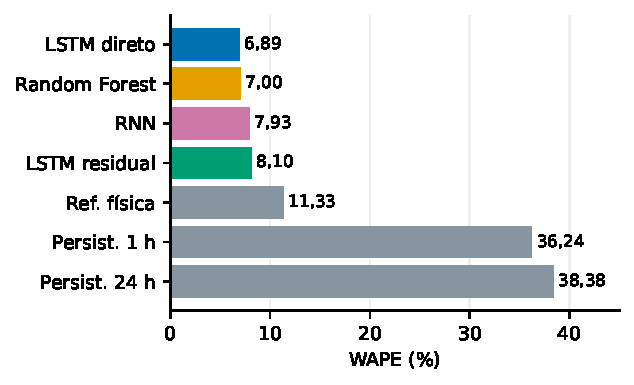
\includegraphics[width=0.75\textwidth]{imagens/fig_wape.pdf}
% \caption{Comparação do WAPE dos modelos. Fonte: resultados V3, dados sintéticos.}
% \label{fig:wape}
% \end{figure}

\begin{figure}[!h]
\centering
\textbf{Fonte:} Elaborado pelo autor.
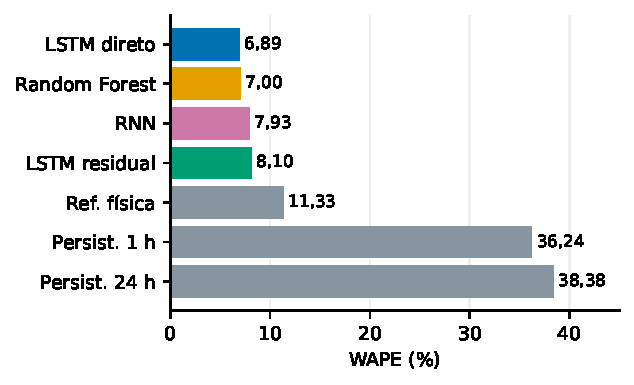
\includegraphics[width=0.75\textwidth]{imagens/fig_wape.pdf}
\caption{Comparação do WAPE dos modelos.}
\label{fig:wape}
\end{figure}

A Figura~\ref{fig:hour} apresenta o primeiro dia completo do teste, 14 de abril de 2025, para a semente 42. O total de referência foi de 28,43 kWh, enquanto o LSTM direto estimou 29,60 kWh e o Random Forest, 29,74 kWh. O gráfico apresenta previsões sucessivas de uma hora à frente, não uma previsão das 24 horas emitida de uma só vez.

\begin{figure}[H]
\centering
\textbf{Fonte:} Elaborado pelo autor.
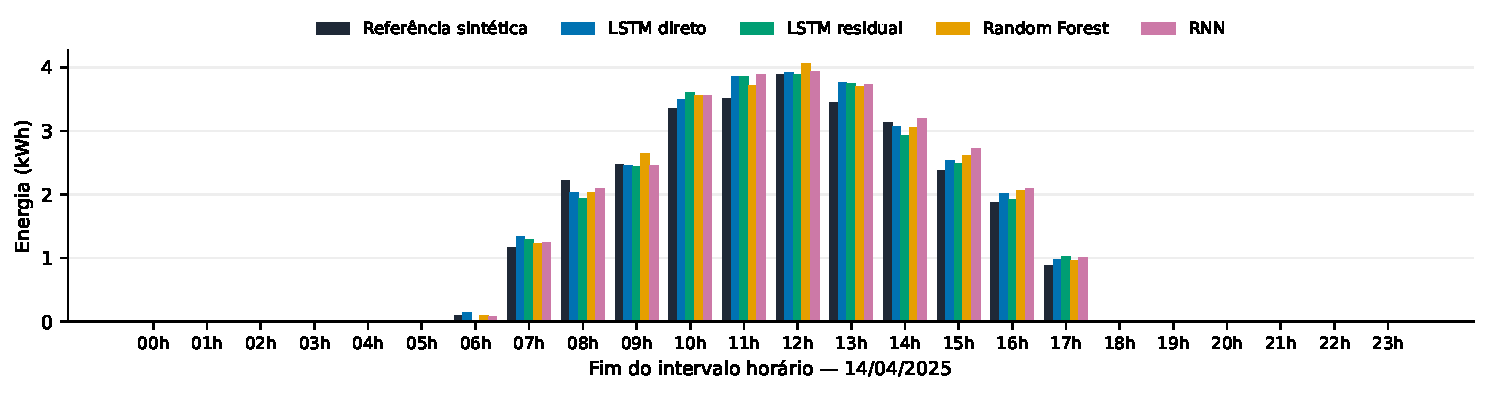
\includegraphics[width=0.99
\textwidth]{imagens/fig_24h.pdf}
\caption{Geração horária sintética e previsões em 14/04/2025, semente 42. Fonte: resultados V3.}
\label{fig:hour}
\end{figure}
% \FloatBarrier
Os resultados também foram examinados em condições meteorológicas específicas. Nos intervalos com chuva prevista, o Random Forest obteve MAE de 0,0613 kWh, ante 0,0828 kWh do LSTM direto. Sob nebulosidade prevista de pelo menos 70\%, os erros foram 0,0628 e 0,0852 kWh, respectivamente. Isso indica que a vantagem global do LSTM não se repetiu em todos os recortes. O erro médio diurno do LSTM direto foi de 0,1055 kWh, superior ao erro global, pois os 198 intervalos noturnos tiveram geração-alvo e previsões iguais a zero. Os erros de teste não constituem garantia de precisão futura.

\subsection{Relação com o estudo de Corrêa}
Em seu trabalho, Corrêa (2026, p. 54--57) \cite{correa} utilizou dados diários de geração de uma instalação do IFES em Linhares, associados à base meteorológica NSRDB. Entre quatro configurações LSTM, o modelo com variáveis meteorológicas ampliadas e codificação sazonal, com janela de três dias, apresentou MAE de 89,53 kWh e MAPE de 30,22\%. O autor observou que janelas de 30 dias não produziram os melhores resultados e discutiu a influência da quantidade e da qualidade dos dados de entrada.

Essa observação reforça a motivação para manter uma arquitetura simples e incluir informações meteorológicas e temporais relevantes neste projeto. Entretanto, os valores de erro dos dois estudos não podem ser comparados diretamente: Corrêa utilizou geração diária medida em uma instalação de porte distinto, enquanto este estudo utilizou geração horária sintética e métricas percentuais diferentes. A janela de 24 horas adotada aqui também não foi comparada com outros tamanhos neste experimento.